\projectname{} simplifies the troubleshooting process by programmatically localizing the root cause
of network problems along three dimensions: {\it what} network problems exist at a
particular point in time, {\it where} in the control software a problem first developed, and
{\it when} the triggering event occurred. In this section we present
the components of \projectname{} we have designed for performing software fault localization for SDN.

\subsection{Correspondence Checking}

The SDN platform transforms high-level policies (specified by the control application) into low-level configuration of they physical infrastructure.
The configuration of the physical network should semantically correspond with the policy specified by the application layer, in the sense that the disposition of any packet by the physical forwarding tables should reflect  the policies dictated for that packet. We refer to any lack of semantic correspondence
between the policy and the configuration as a {\it policy-violation}.

We leverage the virtual packet algebra pioneered in headerspace
analysis~\cite{hsa} to verify whether the application's policies are indeed
implemented correctly in the physical network. Our algorithm, correspondence
checking, provides a crisp determination of all possible packet inputs that
would not behave according to the application's policies if injected into the
network at a particular point in time. Furthermore, running correspondence
checking between intermediate layers of the SDN stack (logical view versus
physical view), allow us to identify the component(s) of
the system where policy-violations first manifest themselves.

Formally, the state of the physical network, the physical view, and the
logical view can be represented as a graph,
$G = (V, E)$. Packets are series of bits, $h \in \{0,1\}^L = H$,
where $L$ is the maximum number of bits in the header.

Upon receiving a packet,
forwarding elements apply a transformation function, potentially modifying
packets before forwarding them on\footnote{Multicast forwarding can expressed
by extending the range to sets of output tuples}:
\begin{align*}
T: (H \times E) \rightarrow (H \times E_{\emptyset})
\end{align*}

We use $`\Psi`$ to denote the collection of all transfer functions present in
the network at a particular point in time. In this model, network traversal is simply a composition of transformation
functions. For example, if a header $h$ enters the network through edge
$e$, its state after $k$ hops will be:
\begin{align*}
\Psi^k(h,e) = \Psi(\Psi(\dots \Psi(h,e)\dots))
\end{align*}

The externally visible behavior of the network can be expressed as the
transitive closure of $\Psi$:
\begin{align*}
\Omega: (H \times E_{access}) \rightarrow (H \times E_{\emptyset}) \\
\Omega(h,e) = \Psi^{\infty}(h,e)
\end{align*}
Here, $E_{access}$ denotes access links adjacent to end-hosts.
In words, $\Omega$ is a mapping between all possible input packets inserted
into the network from an end-hosts, to the final location of the packet after
traversing the network.

In SDN, it should always be the case that:
\begin{align*}
\Omega^{view} \sim \Omega^{physical}
\end{align*}
Informally, this means that any packet injected at an access link in $G^{virtual}$ should arrive at
the same final location as the corresponding (encapsulated) packet injected at the
corresponding access link in $G^{physical}$. Note that hosts are represented
in all layers, although there may not be a one-to-one mapping between the
internal vertices of $G^{virtual}$ and $G^{physical}$.

To check correspondence in SDN, we begin by taking a causally consistent
snapshot~\cite{Chandy:1985:DSD:214451.214456} of the physical network. The routing
tables of forwarding elements can then be translated into transformation functions.
Finally, we feed a symbolic packet $x^L$ to each access link of the
network.\footnote{The rules for process wildcard bits $x^n$ are defined in
the HSA paper~\cite{hsa}} The end result is a propagation graph representing all possible paths taken by a packet injected
at the access link.

The leaves of the propagation graph represent $\Omega$. We
verify correspondence in SDN by generating propagation graphs for all SDN layers,
and comparing the leaves. Any mismatch in leaves of the propagation graphs
represent policy-violations between control applications and network
configuration.

It is important to note that correspondence checking assumes that the
application's policies are correct; it only checks whether the physical
network's configuration is isomorphic with the logical view, but does not
check for additional correctness properties such as connectivity and
loop-free routing. If the user wishes to explicitly express additional
invariants, the HSA framework used by our system can
easily check for such properties.

\subsection{\SIMULATOR{}}

Correspondence checking infers all policy-violations in the network at a
particular point in time. However, troubleshooters
need two additional pieces of the diagnostic puzzle.

First, in large distributed
systems with communication delay and hardware failures, transient policy-violations
are unavoidable, even common. That is, every time there has been a link failure that the SDN platform has not had time to respond to, or every time there has been a policy change that has not yet propagated down to the physical switches, there is a policy-violation.  Most of these policy violations will be temporary, resolving as soon as the SDN platform has had time to respond.  Some of these policy violations will persist, and that indicates a problem in the SDN platform.  In addition, even some of the ephemeral violations may be harmful (such as those that violate isolation conditions), which again indicate a problem in the SDN platform.

Troubleshooters therefore need a mechanism to differentiate
policy-violations that indicate a problem in the SDN platform from those that merely reflect inherent delays in responding to events; we will call all policy-violations that indicate a problem``pernicious'' violations.

Second, once pernicious policy-violations are encountered, troubleshooters need to
identify the events (link failures, controller failures, VM migrations,
\etc{}) that triggered the problem. Moreover, they would like to have these events narrowed down to a minimal set, to make it easier to understand the problem.

\Simulator{} is our mechanism for providing this information. \Simulator{} models
the network in a single simulation process, thereby providing arbitrary control over hardware
failures, message delays and other failure modes. \Simulator{} distinguishes
between ``internal'' events that happen throughout the normal course of the
system execution (\eg{} message sends and receives), and ``external'' events
injected into the system (\eg{} link failures). We describe the details
of the simulator in the next section.

The key insight behind
\simulator{} is that fault localization is significantly easier with the
ability to selectively filter
out external events from the system execution and observing how the system
plays out in isolation.
With complete control over the
system execution, we are able to programmatically (i) track the lifetime of
policy-violations to differentiate persistent from transient errors, and (ii)
infer the `minimal causal set' of events triggering the problem. We describe
these components below.

Note that we have implemented policy-violation lifetime tracking, but we are
still developing the infrastructure for minimal causal set inference.
Nonetheless, we present our algorithm in this section.

\subsubsection{Policy-Violation Lifetime Tracking} The first step in
\simulator{} involves detecting policy-violations and prioritizing them based
on their duration.
We do so in a relatively straightforward fashion. First, we take as input
a stream of network events (\eg{} link failures). Event sequences are either
synthetically generated or gathered from a production trace of failure and topology change
events, as enabled, \eg{}, by OFRewind~\cite{ofrewind}. We then replay the execution of the
control plane based on the input trace. Throughout the system execution,
the simulator periodically invokes correspondence checking to enumerate all
policy-violations (defined as any value in $\Omega^{physical}$ not present in
$\Omega^{virtual}$, or vice versa). When a policy-violation is detected,
the simulator forks off a branch that investigates the future system behavior
in a case where no further failure events are played out. Finally, we
prioritize the policy-violations based on their duration.

\subsubsection{\bf Causal Inference} Having identified persistent
policy-violations, \simulator{} seeks to identify the `minimal causal set' of
events leading up to the problem. By `minimal causal set', we mean
the minimally-sized set of events preceding (defined by the `happens-before'
relation~\cite{Lamport:1978:TCO:359545.359563}) the onset of the policy-violation, such that
if any single event were removed the set, the policy-violation would not have resulted.
% * would not have resulted *in such a long duration event*?

\Simulator{} captures the notion of causality by attaching vector clocks~\cite{Mattern89virtualtime} to
all control messages in the simulated execution of the system. Our
simulator runs as a single sequential thread; therefore we convert any partially-ordered input trace
of network events into a totally-ordered trace by choosing an arbitrary
sequential ordering that maintains the `happens-before'
relation.

Without regarding casual constraints, a naive algorithm to infer the minimal
causal set would be to iteratively
exclude each event from the system execution, and see if the policy-violation
still appears. The problem is that we cannot simply ``erase history'';
antecedent events in the system execution may have depended on the event we
are excluding.

Our algorithm therefore proceeds as as follows. First, consider
the state of the system at exactly the point where the given policy-violation
occurs. The active `causal branches' in the system at this time are (i) the
most recent event (message send, message receive, or internal state change)
occurring on every node in the system, and (ii) the message send event for any
in-flight control packets in the network. Our goal is to prune these causal
branches until we are left with the minimal causal set at the leaves of the
pruned branches.

%\begin{figure}[t]
%    %\hspace{-10pt}
%    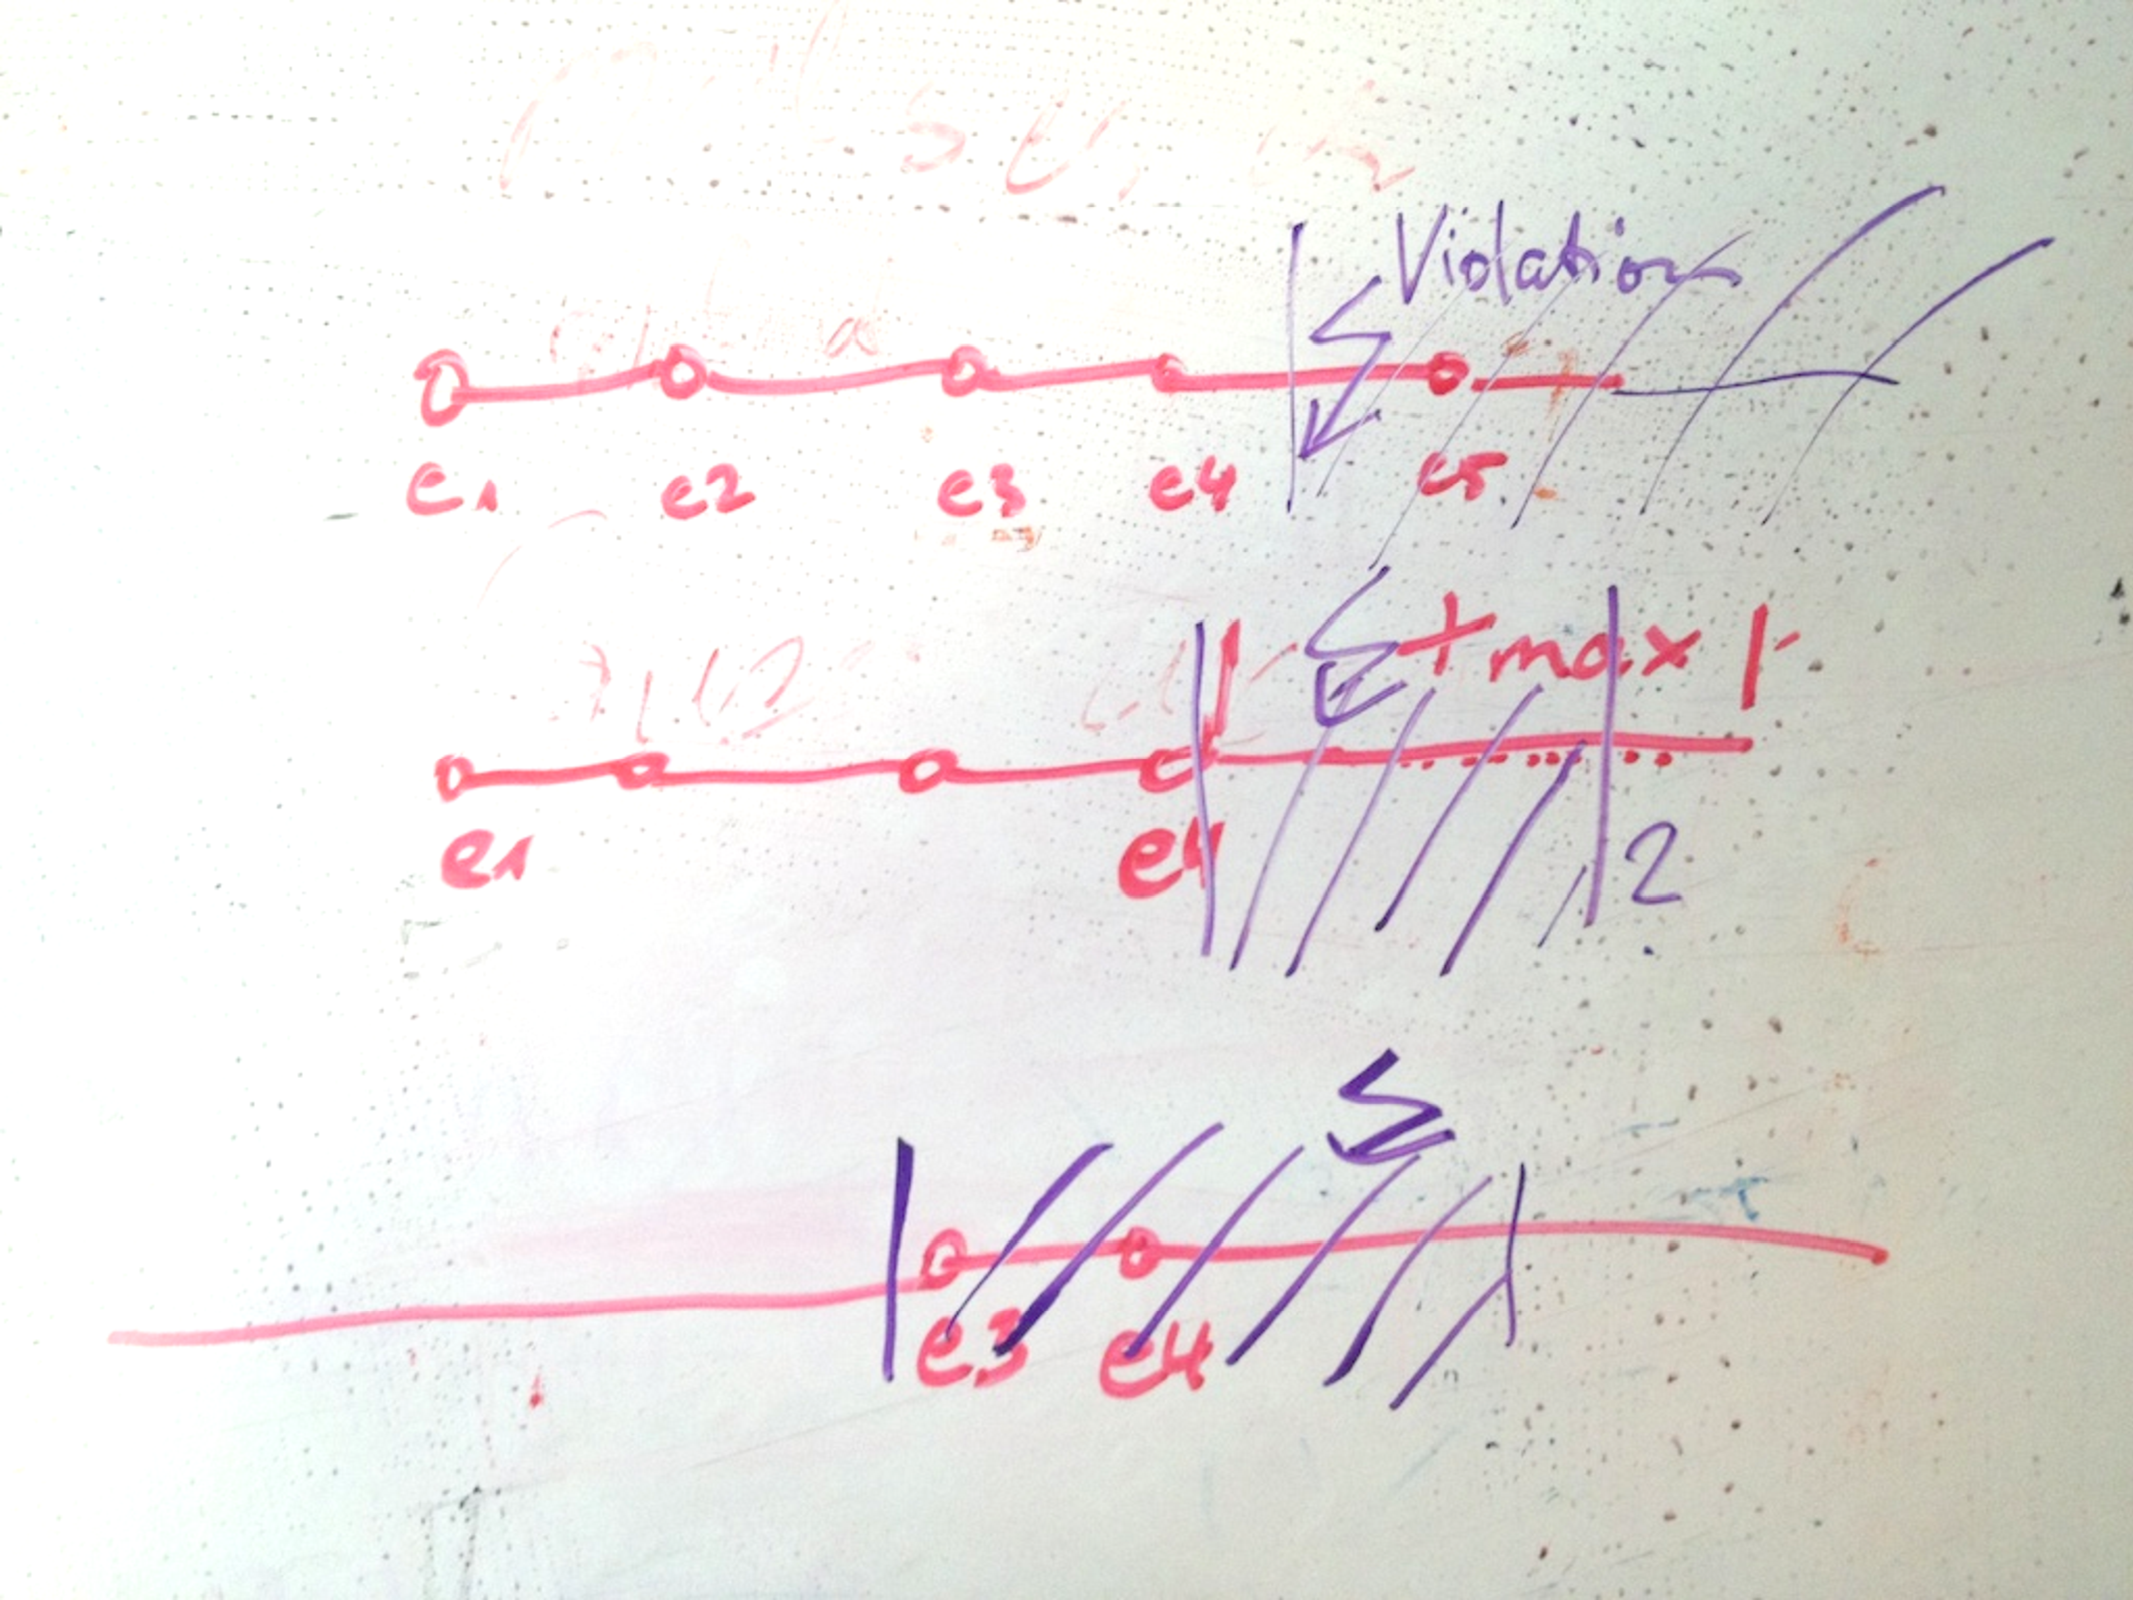
\includegraphics[width=3.25in]{../diagrams/approach/localizing}
%    \caption[]{\label{fig:localizing} Localizing the minimal causal sequence for a failure in the
%    event stream}
%\end{figure}

After having identified the active `casual branches' in the system at the
onset of the policy-violation, our algorithm essentially performs a
traversal of the causal graph's (a DAG) topological ordering, pruning leaves that are not
responsible for the policy-violation. In pseudo-code:

\begin{algorithmic}
\State $causalSet \gets []$
\While {$\exists\;\text{\it leaf in causalGraph}$}
    \State {\it remove leaf from causalGraph}
    \State $violation \gets runSimulation(causalGraph)$
    \If {\it not violation}
        \State $causalSet\;+= leaf$
    \EndIf
\EndWhile
\end{algorithmic}

Here, $runSimulation(DAG)$ executes the system from the beginning of the
trace, and checks whether the policy-violation occurs at the end of the
execution. The beginning of the trace starts at some pre-defined point where
the system was known to be in a coalescent state.

\colin{
Panda and I realized that the minimal casual set algorithm we presented in the OSDI submission is erroneous.

A few things are wrong with this:
\begin{itemize}
\item We can't remove elements of the MCS from the DAG! We should only remove from the DAG if the event is not in the MCS; otherwise, the policy-violation will never be reproduced after the first element is added the MCS, since we took away one of the necessary conditions.
\item Need to make a distinction between "random events" (e.g. link failures, node failures) and "deterministic events" (e.g., a node is programmed to send a pong when it receives a ping). In the MCS algorithm, it makes no sense to prune out deterministic events... However, the algorithm still needs to take in the entire casual DAG (both random and deterministic) to maintain casual dependencies [can't prune arbitrary random events]
\item We assume that the random events are independent; we need make this
assumption explicit. But because we assume they are completely independent,
and because we only manipualate random events, there is no need for vector
clocks!!
\end{itemize}
}

Note that each iteration of the loop can be performed in parallel by cloning
the state of the simulator. The serial runtime of the algorithm is therefore
linear with the number of events in the input trace.

We also note that Lamport's definition of the `happens-before' relation is
conservatively general, and can include events that are not in fact
casually-related. In fact, as described here, our algorithm can be viewed as a
generalization of dependency graph algorithms for hardware fault
isolation~\cite{577079}. In future work we hope to leverage domain
knowledge of network control plane
protocols to provide a more specific definition of causality (\eg{} OpenFlow
control messages with differing transaction ids are not causally related),
allowing us to further prune events that are not in fact causally related from the DAG.

\subsubsection{Additional Use-Cases} Besides lifetime tracking and causal analysis, our simulation infrastructure has a
number of other possible use-cases:

\noindent\textbf{Checking related problems by fuzzing.} Input traces can be \emph{fuzzed}, i.e.,
randomly perturbed, to expose the system to similar error conditions, and confirm
that a proposed solution is not just a point-fix.

\noindent\textbf{Investigating pathological environment conditions.} The simulator allows for investigation
of pathological environment conditions difficult to achieve in a real world test bed
(\eg{}, correlated failure rates, extremely long delays etc.). This enables
investigation of situations that have a high potential for triggering errors.

\noindent\textbf{Interactive exploration.} Troubleshooters can also interactively bisect
the trace or modify specific events to further pinpoint the cause for a failure.
This is useful as soon as a suspect event sequence has been identified.

\noindent\textbf{Regression/Integration Test Library.} In traditional software engineering practices,
integration tests are an
important part of the software development cycle: developers feed end-to-end
input through the system, and verify that the system execution satisfies
certain safety and liveness properties. As additional failure cases are encountered in
production, new cases can be added to a suite of integration tests to
ensure robust operation of the system in future versions of the system.

Although the practice of accumulating an integration test suite over time is
commonplace in other fields of computer science, the field of networking
simply did not have the requisite software infrastructure to realize this practice before the emergence
of SDN. \Simulator{} can be viewed as our realization
of this development practice, applied to network controllers. Our simulator's fine-grained control over
failure scenarios allows us to test corner-case network conditions -- those
that are most difficult to anticipate in traditional unit tests.
As known failure cases are accrued over time, we envision \simulator{} being used to validate
new and existing SDN platforms.

\subsection{Discussion}

Correspondence checking and \simulator{} serve to isolate the platform layer and
event sequence responsible for a given error. \projectname{} can be
complemented by classical debugging techniques (\eg{} log messages and source
code debugging) to identify the root cause of
the failure in the code. These techniques are much more
effective when applied a specific event sequence. Once a
potential fix has been developed, it can be validated by repeating the
problematic execution within \projectname{}. Input fuzzing further helps to
validate whether there are
related error events that the patch missed.
